\documentclass{article}
\usepackage[utf8]{inputenc}
\usepackage{graphicx}
\usepackage{grffile}
\usepackage{float}
\usepackage{amsmath}
\usepackage[margin=1.25in]{geometry}
\usepackage{subfig} 

\title{COVID-19 Pandemic \& Machine Learning}
\author{Khushbu Mevada (MIT2019086) \and Shivam Kasat (MIT2019024) }

\date{04 May 2020}

\begin{document}

\maketitle
\section*{Abstract}
The current research proposes a model to predict the number of people that may be affected, the peak period and the halt time for the coronavirus pandemic outbreak worldwide. Here, we apply Machine learning models to predict aforementioned predictions. We use the statistical data generated from countries, namely India, Spain and South Korea and we also use the statistical data from some of the Indian states for prediction purposes in order to get some meaningful insights from our analysis. 

\section*{Introduction}
\textbf{What is coronavirus?}
\\Coronaviruses are a large family of viruses which may cause illness in animals or humans.  In humans, several coronaviruses are known to cause respiratory infections ranging from the common cold to more severe diseases such as Middle East Respiratory Syndrome (MERS) and Severe Acute Respiratory Syndrome (SARS). The most recently discovered coronavirus causes coronavirus disease COVID-19.
\begin{center}
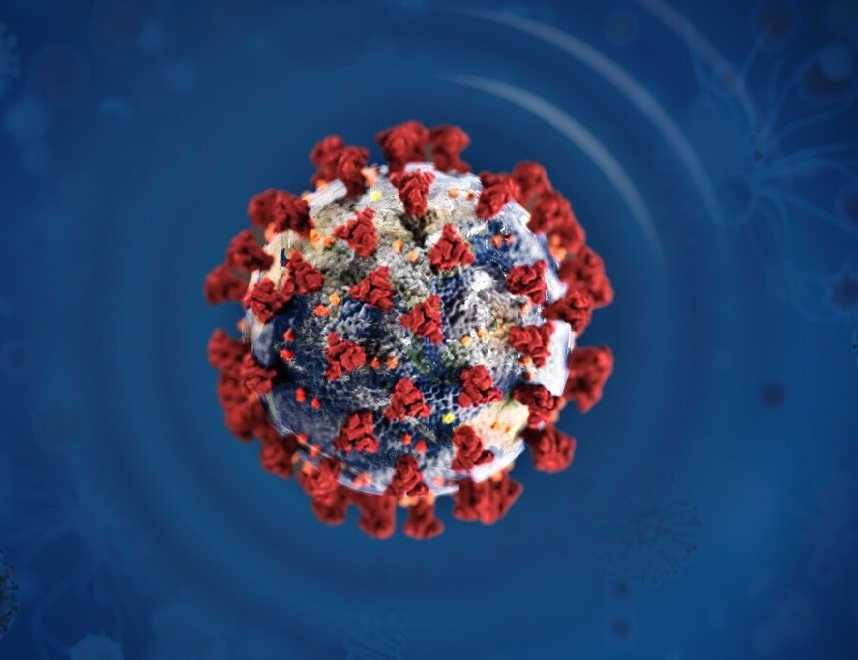
\includegraphics[scale=0.3]{corona_0.jpeg}\newline
\end{center}
COVID-19 is the infectious disease caused by the most recently discovered coronavirus. This new virus and disease were unknown before the outbreak began in Wuhan, China, in December 2019.\newline
\\The first case of 2019-2020 coronavirus pandemic in India was reported on $30^{th}\:$ January, 2020, Originating from China.  
Experts suggest the number of infections could be much higher as India's testing rates are among the lowest in the world. The infection rate of COVID-19 in India is reported to be 1.7, significantly lower than in the worst affected countries.\newline
\clearpage
\textbf{Symptoms of Coronavirus}
\begin{center}
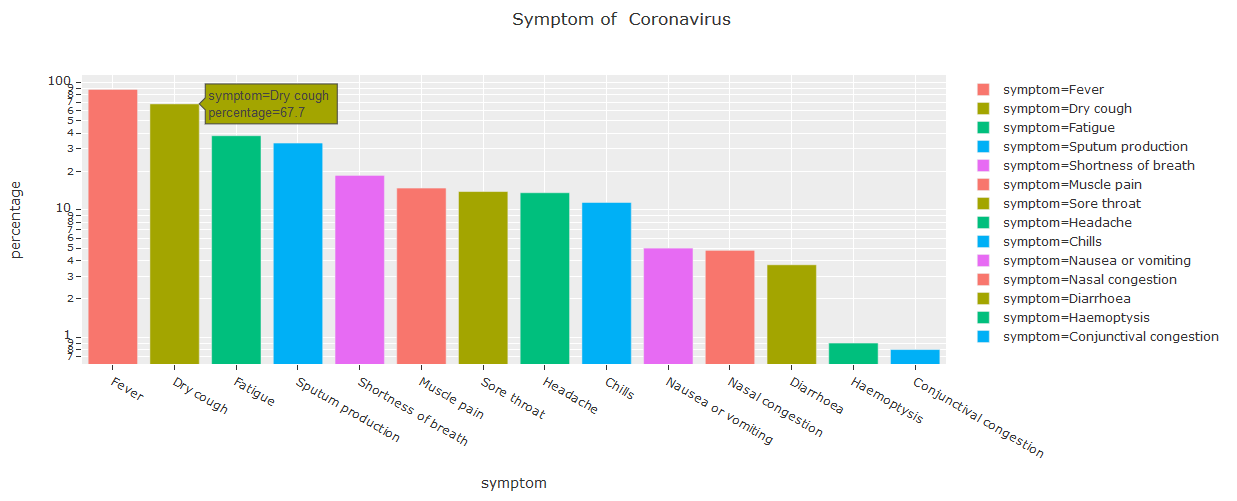
\includegraphics[scale=0.5]{corona_1_symptoms.png}
\end{center}
The above graph represents the probability of having corona positive given the symptom. e.g., There is 67.7\% probability for a person to be tested positive given he has dry cough as a symptom.

\section*{Datasets}
We have used multiple dataset for our analysis and prediction task, which were taken from kaggle.com
\begin{itemize}
\item \textbf{COVID19 GLOBAL Forecast}
\newline
\\The White House Office of Science and Technology Policy (OSTP) pulled together a coalition research groups and companies (including Kaggle) to prepare the COVID-19 Open Research Dataset (CORD-19) to attempt to address key open scientific questions on COVID-19. Those questions are drawn from National Academies of Sciences, Engineering, and Medicine’s (NASEM) and the World Health Organization (WHO).
\\It has six columns named Id, Province state, Country Region, Date, Confirmed Cases, Fatalities.
\\They are currently updating the data daily.

\item \textbf{COVID-19 in India}
\newline
\\This dataset has information from the states and union territories of India at daily level. State level data comes from Ministry of Health \& Family Welfare. Individual level data comes from \textbf{covid19india.}
\begin{itemize}
\item COVID-19 cases at daily level is present in covid\_19\_india.csv file.
\item Individual level details are present in IndividualDetails.csv file.
\item Population at state level is present in population\_india\_census2011.csv file.
\item Number of COVID-19 tests at daily level in ICMRTestingDetails.csv file.
\item Number of hospital beds in each state in present in HospitalBedsIndia.csv file.
\end{itemize}
\item \textbf{Novel Corona Virus 2019 Dataset}
\newline
\\This dataset has daily level information on the number of affected cases, deaths and recovery from 2019 novel coronavirus. Please note that this is a time series data and so the number of cases on any given day is the cumulative number.
\\Main file in this dataset is covid\_19\_data.csv and the detailed descriptions are below.
\begin{itemize}
\item Sno - Serial number
\item ObservationDate - Date of the observation in MM/DD/YYYY
\item Province/State - Province or state of the observation (Could be empty when missing)
\item Country/Region - Country of observation
\item Last Update - Time in UTC at which the row is updated for the given province or country. 
\item Confirmed - Cumulative number of confirmed cases till that date
\item Deaths - Cumulative number of of deaths till that date
\item Recovered - Cumulative number of recovered cases till that date
\end{itemize}
\end{itemize}

\section*{Exploratory Data Analysis (EDA)}
\subsubsection*{EDA on COVID19 GLOBAL Forecast dataset}
\begin{itemize}
\item
The dataset covers 163 countries and almost 2 full months from 2020, which is enough data to get some clues about the pandemic. We will see a few plots of the worldwide tendency to see if we can extract some insights:
\begin{center}
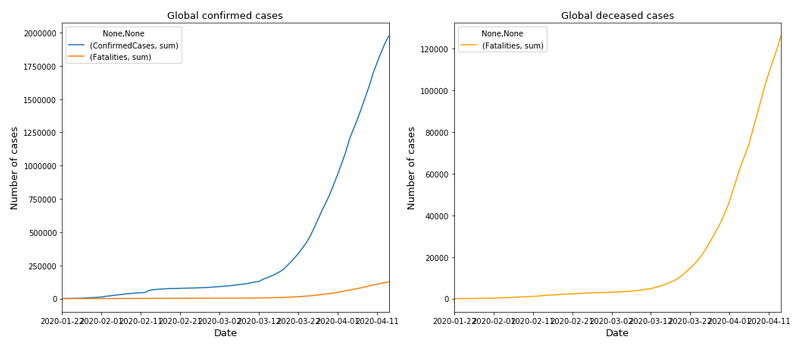
\includegraphics[scale=0.70]{corona_2_global_cases}
\end{center}
\textbf{Observation:}
\\We can see that the global curve shows rich fine structure, but these numbers are strongly affected by the vector zero country, China. Given that COVID-19 started there, during the initial expansion of the virus there was no reliable information about the real infected cases.
\item
Both Italy and Spain are experiencing the larger increase in COVID-19 positives in Europe. At the same time, UK is a unique case given that it's one of the most important countries in Europe but recently has left the European Union. The fourth country we have taken is Singapore, since it is closer to China and its socio-economic conditions is different from the other three countries.
\begin{center}
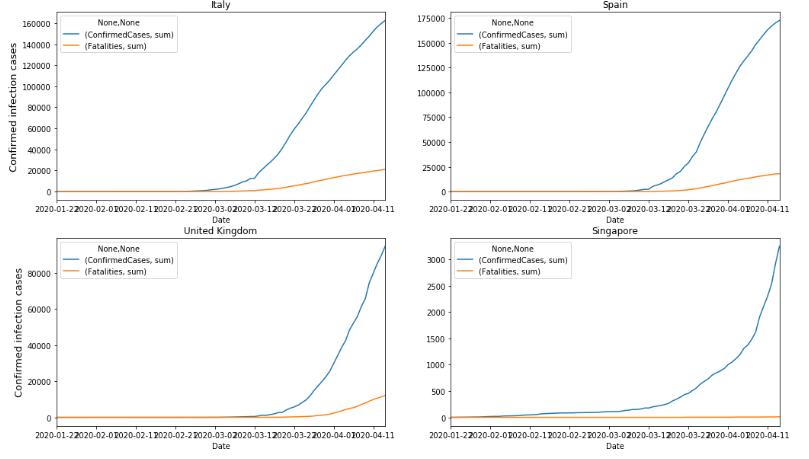
\includegraphics[scale=0.60]{corona_3_countries.png}
\end{center}
\begin{center}
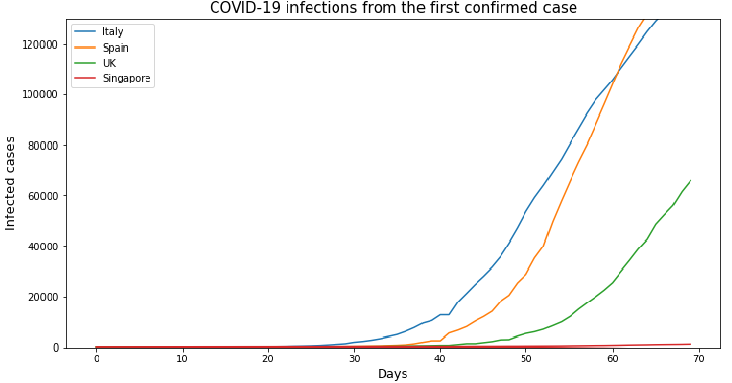
\includegraphics[scale=0.70]{corona_4_countries.png}
\end{center}
\textbf{Observations:}
\begin{itemize}
\item \textbf{Italy}
\\With almost 120,000 confirmed cases, Italy shows one of the most alarming scenarios of COVID-19  with more than 2\% of population has been infected.
\item \textbf{Spain}
\\Spain has the same number of cumulative infected cases as Italy, near 120,000. However, Spain's total population is lower (around 42 millions) and hence the percentage of population that has been infected rises up to 3\%.
\item \textbf{United Kingdom}
\\Despite not being very far from them, the UK shows less cases. The number of cases is around 40.000, this is, a 0.6\% of the total population.
\item \textbf{Singapore}
\\Singapore is relatively isolated given that is an island, and the number of international travels is lower than for the other 3 countries. The number of cases is still very low (<1000) with 0.2\% of population being infected.
\end{itemize}
\end{itemize}
\subsubsection*{EDA on COVID-19 INDIA dataset}
\begin{itemize}
\item The following table shows the details like total number of confirmed cases, number of recovered cases, deaths, active cases, mortality rate for all the states/union territories having active cases till date $4^{th}\:$May, 2020.
\begin{center}
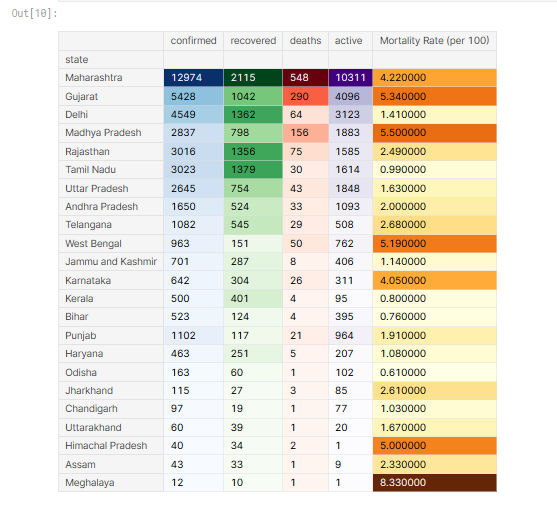
\includegraphics[scale=0.75]{corona_10_states}
\end{center}
\item Top 10 most affected states of India with confirmed number of cases till date $4^{th}\:$May, 2020.
\begin{center}
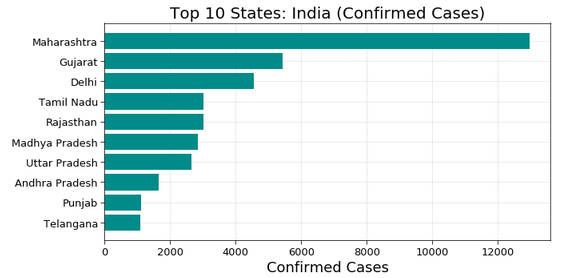
\includegraphics[scale=0.75]{corona_11_topstates}
\end{center}
\end{itemize}

\section*{Prediction}
\subsubsection*{Preprocessing data}
\begin{itemize}
\item \textbf{Join data.}\\ Join train/test to facilitate data transformations
\item \textbf{Filter dates.} \\  remove ConfirmedCases and Fatalities post 2020-03-12. Create additional date columns
\item \textbf{Missing values.} \\Analyze and fix missing values
\end{itemize}
\subsubsection*{Compute lags and trends}
\begin{itemize}
\item \textbf{Lag}
\\Lags are a way to compute the previous value of a column, so that the lag 1 for ConfirmedCases would inform the this column from the previous day. The lag 3 of a feature X is :
\begin{align*}
X_{lag3} (t) = X(t - 3)
\end{align*}
\item \textbf{Trend}
\\Transformig a column into its trend gives the natural tendency of this column, which is different from the raw value. The definition of trend we applied is:
\begin{align*}
Trend_X = \frac{X(t) - X(t-1)}{X(t-1)}
\end{align*} 
\end{itemize}
The backlog of lags we applied is 14 days, while for trends is 7 days.
\subsubsection*{Add country details}
Variables like the total population of a country, the average age of citizens or the fraction of people living in cities strongly impact on the COVID-19 transmission behavior. so, we added those details to data.
\subsubsection*{Linear regression model for prediction}
\begin{enumerate}
\item \textbf{Features.} Select features
\item \textbf{Dates.} Filter train data from 2020-03-01 to 2020-03-20
\item Begin with the train dataset, with all cases and lags reported
\item Forecast only the following day, through the Linear Regression
\item Set the new prediction as a confirmed case
\item Recompute lags
\item Repeat from step 4 to step 6 for all remaining days 
\end{enumerate}
\clearpage
\textbf{Observations:}
\begin{itemize}
\item \textbf{India}
\begin{center}
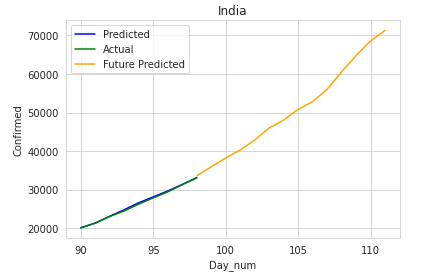
\includegraphics[scale=0.5]{corona_6_india.png}
\end{center}
\item \textbf{Spain}
\begin{center}
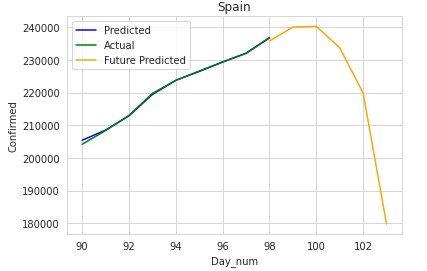
\includegraphics[scale=0.5]{corona__5_spain.png}
\end{center}
\item \textbf{South Korea}
\begin{center}
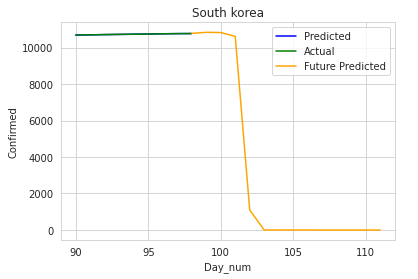
\includegraphics[scale=0.5]{corona_7_southkorea.png}
\end{center}
\item \textbf{Kerala}
\begin{center}
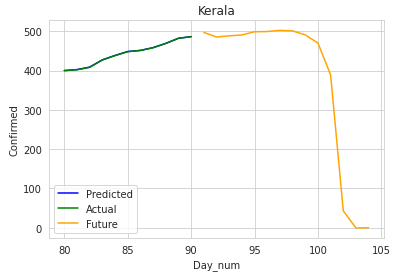
\includegraphics[scale=0.5]{corona_8_kerala.png}
\end{center}
\end{itemize}
\clearpage
\section*{Prevention}
To avoid the critical situation people are suggested to do following things
\begin{itemize}
\item Avoid contact with people who are sick.
\item Avoid touching your eyes, nose, and mouth.
\item Stay home when you are sick.
\item Cover your cough or sneeze with a tissue, then throw the tissue in the trash.
\item Clean and disinfect frequently touched objects and surfaces using a regular household
\item Wash your hands often with soap and water, especially after going to the bathroom; before eating; and after blowing your nose, coughing, or sneezing. If soap and water are not readily available, use an alcohol-based hand sanitizer.
\end{itemize}

\section*{Conclusion}
From the above mentioned graphs we can conclude that according to our linear regression model 
\begin{itemize}
\item the peak on pandemic in \textbf{India} may come after almost 110 days.
\item the peak on pandemic in \textbf{Spain} may come between 95-100 days and will finished after 105 days.
\item the peak on pandemic in \textbf{South Korea} may come between 98-102 days and will finished after 110 days.
\item the peak on pandemic in state  India, named\textbf{Kerala} may come between 85-90 days and will finished after 110 days.

\end{itemize}
\clearpage
\section*{References}
\begin{enumerate}
    \item https://www.who.int/news-room/q-a-detail/q-a-coronaviruses
    
    \item https://www.kaggle.com/c/covid19-global-forecasting-week-4
    
    \item https://www.kaggle.com/sudalairajkumar/novel-corona-virus-2019-dataset
    
    \item https://www.kaggle.com/sudalairajkumar/covid19-in-india
    \item https://towardsdatascience.com/time-series-machine-learning-regression-framework-9ea33929009a
    \item https://towardsdatascience.com/global-covid-19-forecasting-with-linear-regression-and-arima-c154c163acc1
\end{enumerate}
\clearpage
\section*{Acknowledgements}
\begin{itemize}
\item
World Health Organization (WHO)
\item
Johns Hopkins University for making the data available for educational and academic research purposes
\item
Indian Ministry of Health \& Family Welfare for making the data available to general public.
\item
covid19india.org for making the individual level details and testing details available to general public.
\item
Wikipedia for population information.
\end{itemize}
\end{document}
